\documentclass[10pt]{article}
\usepackage{icmlko}

\icmlmeta{IP 파운데이션 월드모델}{91}{어느 카테고리에 쓸 수 있나}{도구를 열 도메인으로 넓히고 자기 검사를 붙였다 --- 성분 수는 전역 상수가 아니었다}

\begin{document}

\twocolumn[
\icmlheader

\begin{abstract}
노트 89의 도구는 팝업 전용이었다. 규약 자체는 도메인을 안 가리므로 열 개
전부로 넓히고 \textbf{자기 검사}를 붙였다 --- 그 도메인의 과거 레코드를 폴드
밖으로 빼고 매겨 순위 상관을 낸다(200건 미만은 하나씩, 그 이상은 10겹).
\textbf{쓸 만한 카테고리와 아닌 카테고리가 갈린다} --- 모바일 $+$0.614 ·
만화 $+$0.483 · \textbf{팝업 $+$0.471} · 세계애니 $+$0.417 · 웹툰 $+$0.387은
쓸 수 있고, 도서 $+$0.180 · 펀딩 $+$0.197은 못 쓴다. 노트 90이 남긴 신호
--- ``팝업만은 성분 $k{=}1$이 낫다'' --- 도 열 도메인에서 확인했다.
\textbf{평균은 같다}($k{=}2$ $+$0.3628, $k{=}1$ $+$0.3531). 그런데 도메인마다
갈린다 --- 팝업 $+$0.021 · 모바일 $+$0.033 · 애니 $+$0.021은 $k{=}1$이 낫고
게임 $-$0.069 · 도서 $-$0.058은 $k{=}2$가 낫다. \textbf{성분 수는 전역 상수가
아니라 도메인의 성질이다.} 도메인마다 좋은 쪽을 고르면 $+$0.3703인데, 열 번의
이지선다라 선택 편향이 섞여 있어 채택하지 않는다(노트 67 · 80). 구현에서 버그도
하나 잡았다 --- 대상만 $k{=}1$로 두면 프로크루스테스 적재의 모양이 안 맞는다.
\texttt{spaces()} 에 성분 수를 뚫었다.
\end{abstract}
]

\begin{figure*}[t]
\centering
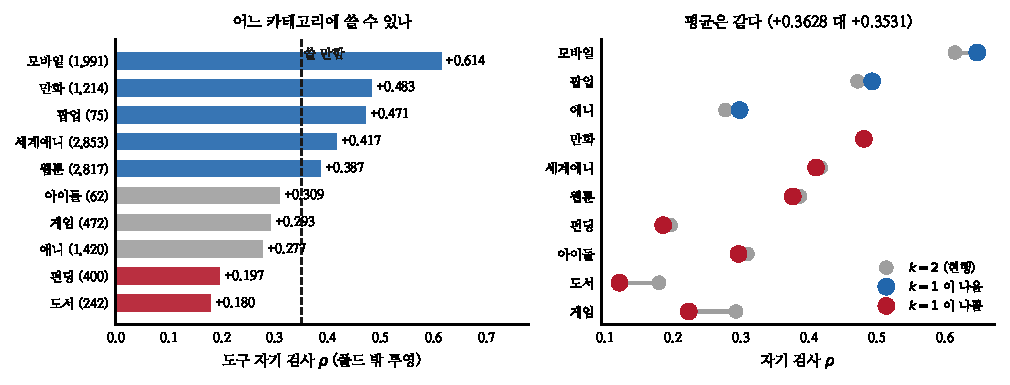
\includegraphics[width=\textwidth]{figs/tk.pdf}
\caption{왼쪽 --- 도메인별 자기 검사. 오른쪽 --- 성분 수 $k{=}1$ 대 $k{=}2$.}
\end{figure*}

\section{도구를 넓혔다}

\begin{quote}\fontsize{9.0}{11}\selectfont\ttfamily
python3 -m state.score --table\\
python3 -m state.score --selftest --domain 웹툰\\
python3 -m state.score --plan plan.json --k 1
\end{quote}

규약은 노트 77의 규약 ④ 그대로다 --- 그 도메인의 과거 레코드로 공간을 만들고
새 레코드 하나를 투영한다. \textbf{자기 검사는 그것을 폴드로 반복한다} ---
200건 미만은 하나씩 빼고, 그 이상은 10겹으로 나눈다(큰 도메인에서 LOO 는
계산이 $n$배라 못 돌린다).

\section{쓸 만한 카테고리}

\begin{table}[t]
\centering\tsize
\caption{도구 자기 검사. 성분 $k{=}2$.}
\begin{tabular}{lrr}
\toprule
& $n$ & $\rho$ \\
\midrule
\textbf{모바일} & 1,991 & \textbf{$+$0.614} \\
만화 & 1,214 & $+$0.483 \\
\textbf{팝업} & 75 & \textbf{$+$0.471} \\
세계애니 & 2,853 & $+$0.417 \\
웹툰 & 2,817 & $+$0.387 \\
\midrule
아이돌 & 62 & $+$0.309 \\
게임 & 472 & $+$0.293 \\
애니 & 1,420 & $+$0.277 \\
펀딩 & 400 & $+$0.197 \\
도서 & 242 & $+$0.180 \\
\bottomrule
\end{tabular}
\end{table}

\claimx{도구를 쓸 수 있는 카테고리와 없는 카테고리가 갈린다. 다섯(모바일 · 만화 ·
팝업 · 세계애니 · 웹툰)은 $\rho\ge+$0.39이고 다섯은 $+$0.31 아래다.}{자기 검사
$\rho$가 파이프라인의 ``대상으로'' 수치보다 낮다(웹툰 $+$0.387 대 $+$0.457).
규약이 더 엄격해서다 --- 인자 공간을 폴드 안에서만 만들고 폴드 밖을 투영한다.
같은 것을 재는 두 숫자가 아니다.}

팝업이 표본 75건으로 셋째다. \textbf{표본 크기가 아니라 축과 라벨의 관계가
성적을 정한다} --- 노트 74의 법칙($r=+$0.99, 자기 상관이 대상 전이를 결정한다)이
도구 수준에서도 보인다.

\section{성분 수는 도메인의 성질이다}

\begin{table}[t]
\centering\tsize
\caption{$k{=}1$ 대 $k{=}2$.}
\begin{tabular}{lrrr}
\toprule
& $k{=}2$ & $k{=}1$ & $\Delta$ \\
\midrule
\textbf{모바일} & $+$0.614 & \textbf{$+$0.647} & $+$0.033 \\
\textbf{팝업} & $+$0.471 & \textbf{$+$0.493} & $+$0.021 \\
\textbf{애니} & $+$0.277 & \textbf{$+$0.298} & $+$0.021 \\
만화 & $+$0.483 & $+$0.481 & $-$0.002 \\
세계애니 & $+$0.417 & $+$0.410 & $-$0.007 \\
웹툰 & $+$0.387 & $+$0.376 & $-$0.011 \\
펀딩 & $+$0.197 & $+$0.186 & $-$0.011 \\
아이돌 & $+$0.309 & $+$0.296 & $-$0.013 \\
도서 & $+$0.180 & $+$0.121 & $-$0.058 \\
게임 & $+$0.293 & $+$0.223 & $-$0.069 \\
\midrule
\textbf{평균} & \textbf{$+$0.3628} & $+$0.3531 & $-$0.010 \\
\bottomrule
\end{tabular}
\end{table}

\claimx{성분 수는 전역 상수가 아니라 도메인의 성질이다. 평균은 $k{=}1$과 $k{=}2$가
$-$0.010밖에 안 다른데 도메인별로는 $+$0.033에서 $-$0.069까지 갈린다.}
{도메인마다 좋은 쪽을 고르면 $+$0.3703이지만 열 번의 이지선다라 선택 편향이
섞인다. 노트 67 · 80이 같은 함정을 보였다 --- \textbf{채택하지 않는다.}}

$k{=}1$이 나은 셋(모바일 · 팝업 · 애니)과 나쁜 둘(게임 · 도서)의 차이가
무엇인지는 모른다. 관측 축 수(게임 6 · 도서 4 · 팝업 5 · 모바일 4)로도,
표본 크기로도 안 갈린다.

\section{버그 하나}

대상 공간만 $k{=}1$로 만들면 프로크루스테스가 $c\times1$ 적재와 $c\times2$
적재를 맞추려다 모양이 안 맞는다. \texttt{spaces()} 가 성분 수를 안 받고 있었고
기본값 2로 고정돼 있었다. 뚫었다.

\begin{quote}\fontsize{9.5}{11.5}\selectfont
설정이 두 곳에 나뉘어 있으면 한쪽만 바뀐다. 노트 65가 진단 코드를 모으고
노트 88이 정직 절차를 코드에 넣은 것과 같은 종류의 정리다.
\end{quote}

\section{한계}

\begin{itemize}[leftmargin=1.1em,itemsep=0.15em]
\item 큰 도메인은 10겹이고 작은 도메인은 하나씩이라 규약이 다르다. 10겹이
      더 낙관적일 수 있다(학습 표본이 90\%).
\item 도메인별 $k$를 고르는 것이 왜 안 되는지(선택 편향)를 계산으로 보이지
      않았다. 씨앗 넷 규약으로 판정하지도 않았다.
\item 자기 검사가 순위만 잰다. 도구가 내는 ``비슷한 자리의 방문자 범위''는
      검사하지 않았다.
\item 도서 · 펀딩이 왜 낮은지 모른다. 축이 얇아서로 보이지만 확인 안 했다.
\item 도구는 여전히 팝업의 열 속성 중 다섯만 쓴다(노트 89 · 90).
\end{itemize}

\section{다음}

\begin{enumerate}[leftmargin=1.3em,itemsep=0.15em]
\item 도메인별 성분 수를 \textbf{씨앗 넷 규약}으로 판정한다. 선택 편향을
      감당할 만큼 큰지 본다.
\item 도서 · 펀딩이 낮은 이유 --- 축이 얇아서인지 라벨이 시끄러워서인지.
\item 도구의 ``방문자 범위''를 검사한다. 순위는 검사했는데 범위는 안 했다.
\item 팝업 표본. 다섯 노트가 같은 곳을 가리킨다(75 · 86 · 87 · 90 · 91).
\end{enumerate}

\vspace{0.6em}
\hrule height 0.3pt
\vspace{0.5em}
{\footnotesize
\textbf{참고문헌}\\[0.3em]
Ben-David, S. et al. (2010). A theory of learning from different domains.
\emph{Machine Learning}, 79(1--2), 151--175.\\[0.15em]
Schoenemann, P. H. (1966). A generalized solution of the orthogonal Procrustes
problem. \emph{Psychometrika}, 31(1), 1--10.\\[0.15em]
Cawley, G. C., Talbot, N. L. C. (2010). On over-fitting in model selection and
subsequent selection bias in performance evaluation. \emph{JMLR}, 11, 2079--2107.\\[0.15em]
Varoquaux, G. (2018). Cross-validation failure: small sample sizes lead to large
error bars. \emph{NeuroImage}, 180, 68--77.\\[0.15em]
Efron, B., Tibshirani, R. J. (1993). \emph{An Introduction to the Bootstrap}.
Chapman \& Hall.
}

\end{document}
